\documentclass[10pt,a4paper]{article}
\usepackage[utf8]{inputenc}
\usepackage{amsmath}
\usepackage{amsfonts}
\usepackage{amssymb}
\usepackage{pgfplots}
\pgfplotsset{compat=1.9}
\usepackage[english]{babel}
\usepackage{fourier}
\usepackage[left=2cm,right=2cm,top=2cm,bottom=2cm]{geometry}

\newcommand*\Eval[3]{\left.#1\right\rvert_{#2}^{#3}}
\title{Algorithms Test 1 Review}
\author{Benjamin Boudra}
\begin{document}
\maketitle
\tableofcontents
\section{EX 1}
\subsection{Prompt}
\subsection{Answer}

\section{EX 2}
\subsection{Prompt}
\subsection{Answer}

\section{EX 3}
\subsection{Prompt}
Use the technique of bounding definite integrals to find the $\Theta$ category for the function.
\begin{equation}
  A (n) = log_2(1) + log_2(2) + log_2(3) + \ldots + log_2(n-1) + log_2(n)
\end{equation}
Actually, you should use the integral bound technique for one equality, and use trivial analysis for the other.
\subsection{Answer}
\subsubsection{Step 1: Draw a graph of the summation and Integral}
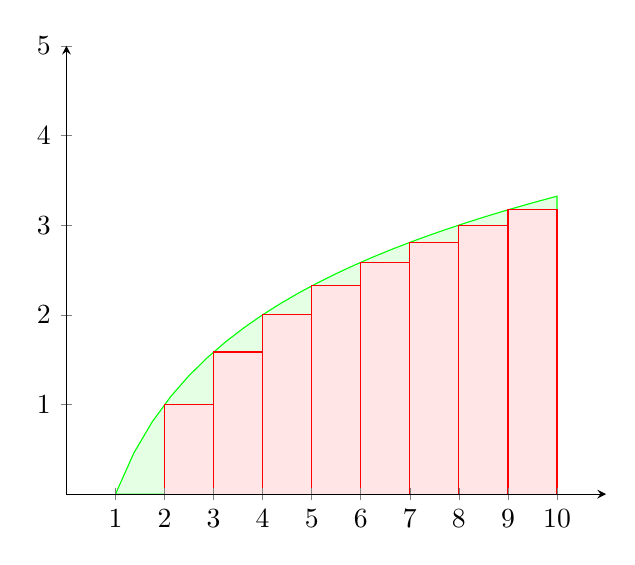
\begin{tikzpicture}
\begin{axis}[
    xtick={0,1,2,3,4,5,6,7,8,9,10},ytick={0,...,10},
    xmax=11,ymax=5,ymin=0,xmin=0,
    enlargelimits=true,
    axis lines=middle,
    clip=false,
    domain=0:11,
    axis on top
    ]

\addplot[draw=green, fill=green!10,domain=1:10]{ln(x)/ln(2)}\closedcycle;
\addplot [draw=red, fill=red!10, ybar interval, samples=10, domain=1:10]
    {ln(x)/ln(2)}\closedcycle;
\end{axis}
\end{tikzpicture}

\subsubsection{Step 2: Deduce the Graph's implications}
Following from the facts that:
\begin{enumerate}
  \item The integral is the area under the function $log_2(x)$ from $1$ to $n$.
  \item If we chose to view the integral as the summation of all of its length one segments from $1$ to $n$ plus the integral of whatever is left over (if n is not an integer value), the resulting integral's value will be unaffected.
  \item The value of each integral segment is greater than the value of its corresponding series segment because:
  \begin{enumerate}
    \item the value of the function and the series are equal at integer values
    \item the value of the function increases between integers and the value of the series does not.
  \end{enumerate}
\end{enumerate}
$\int_1^n log_2(x)$ is greater than $\sum_{i = 1}^n log_2(i)$ for any $n$ greater than $1$. Thus, to find the upper bound or $O$ of $\sum_{i = 1}^n log_2(i)$ we merely need to find the integral of $\int_1^n log_2(x)$\\\\
\subsubsection{Step 3: Calculate the Definite integral}
So now I will calculate $\int_1^n log_2(x)$
\begin{enumerate}
  \item Recognize that to take the integral of a logarithm, we will have to perform integration by parts. so we must chose $u$ and $dv$ values.
  \begin{equation}
    u = log_2(x)\qquad du = 1/xln(2) \qquad dv = 1 \qquad v = x
  \end{equation}
  \item solve for the indefinite integral
  \begin{multline}
    \int_1^n log_2(x) = \Eval{\frac{ln(x)*x}{ln(2)}}{1}{n}- \int_1^n \frac{x}{xln(2)} = \Eval{\frac{ln(x)*x}{ln(2))}}{1}{n} - \int_1^n \frac{1}{ln(2)} = \Eval{\frac{ln(x)*x}{ln(2)} - \frac{x}{ln(2)}}{1}{n} = \\ \Eval{\frac{ln(x)*x-x}{ln(2)}}{1}{n}
  \end{multline}
  \item solve for the definite integral
  \begin{equation*}
    \Eval{\frac{ln(x)*x-x}{ln(2)}}{1}{n} = \frac{ln(n)*n-n}{ln(2)} - \left(\frac{ln(1)*1-1}{ln(2)}\right) = \frac{ln(n)*n-n}{ln(2)} + \left(\frac{1}{ln(2)}\right) = \frac{ln(n)*n-n + 1}{ln(2)}
  \end{equation*}
\end{enumerate}
Thus, The equation:
\begin{equation*}
  \frac{ln(n)*n-n + 1}{ln(2)}
\end{equation*}
Acts as an upper bound for the summation.
\subsubsection{Step 4: Prove Upper Bound is in $\Theta(n log(n))$}
\begin{enumerate}
  \item prove equation is $O(n log(n))$.
  According to our notes, an equation of the category $O(n)$ when it
  \begin{equation}
  \end{equation}
  \item
\end{enumerate}

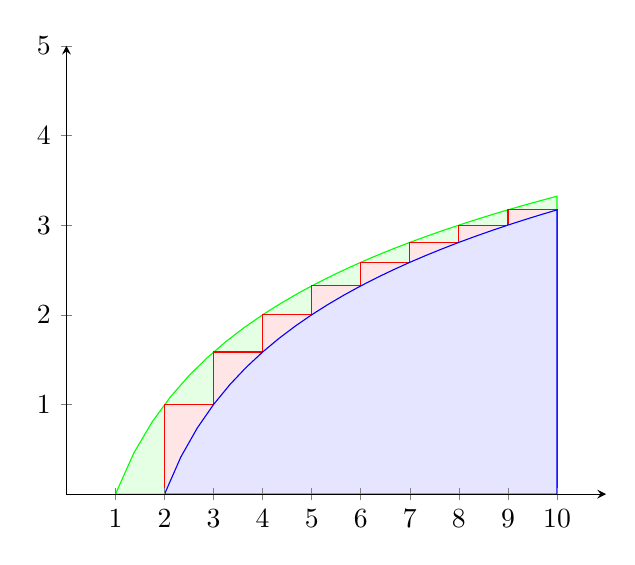
\begin{tikzpicture}
\begin{axis}[
    xtick={0,1,2,3,4,5,6,7,8,9,10},ytick={0,...,10},
    xmax=11,ymax=5,ymin=0,xmin=0,
    enlargelimits=true,
    axis lines=middle,
    clip=false,
    domain=0:11,
    axis on top
    ]
\addplot[draw=green, fill=green!10,domain=1:10]{ln(x)/ln(2)}\closedcycle;
\addplot [draw=red, fill=red!10, ybar interval, samples=10, domain=1:10]
    {ln(x)/ln(2)}\closedcycle;
\addplot[draw=blue, fill=blue!10,domain=2:10]{ln(x-1)/ln(2)}\closedcycle;
\end{axis}
\end{tikzpicture}
\section{EX 4}
\subsection{Prompt}
\subsection{Answer}

\section{EX 5}
\subsection{Prompt}
\subsection{Answer}

\section{EX 6}
\subsection{Prompt}
\subsection{Answer}

\section{EX 7}
\subsection{Prompt}
\subsection{Answer}

\end{document}
